
\RequirePackage[l2tabu, orthodox,danish]{nag}

%%%% Tekst, billeder og sprog %%%%
\documentclass[12pt]{article} 
\usepackage[danish]{babel}
\usepackage[utf8]{inputenc}
%%Billeder%%
\usepackage{graphicx}
\usepackage{float}
\usepackage{microtype}
\usepackage[a4paper,margin=1in,footskip=0.4in,heightrounded]{geometry}
\usepackage{lastpage}
\usepackage{setspace}
\usepackage[explicit]{titlesec}
\usepackage{textcomp}
\usepackage{siunitx}
\usepackage{fancyhdr}
\pagestyle{fancy}
\fancyhf{}
\rhead{\today} 
\lhead{Simon Rumle Tarnow, Daniel Muff Laporte \\Christoffer Irvall Rasmussen, D og P TK1} 
\renewcommand\thesection{\arabic{section}}
% \renewcommand\thesubsection{\thesection.\alph{subsection}}
\rfoot{Side \thepage \hspace{1pt} af \pageref{LastPage}}
\renewcommand{\headrulewidth}{0.1pt}

% %%%% Tabeller  %%%% %
\usepackage[normalem]{ulem}
\useunder{\uline}{\ul}{}



%%%% Referencer %%%%
\usepackage{csquotes}
\usepackage[
backend=biber,
% natbib=true,
style=numeric, 
dateabbrev = false, 
urldate = long, 
date = long
% sorting = anyt
]{biblatex}
\usepackage[colorlinks=false, pdfborder={0 0 0}]{hyperref}
\usepackage[danish]{cleveref}
\usepackage{xpatch}
\addbibresource{files/references/references.bib}
\usepackage{pdfpages}
\usepackage{autonum}
%%%% Math %%%%%
\usepackage{amsmath}
\usepackage{siunitx}
%\def\align@preamble{%
%   &\hfil
%    \setboxz@h{\@lign$\m@th\displaystyle{##}$}%
%    \ifnum\row@>\@ne
%    \ifdim\ht\z@>\ht\strutbox@
%    \dimen@\ht\z@
%    \advance\dimen@\minalignvsep
%    \ht\strutbox\dimen@
%    \fi\fi
%    \strut@
%    \ifmeasuring@\savefieldlength@\fi
%    \set@field
%    \tabskip\z@skip
%   &\setboxz@h{\@lign$\m@th\displaystyle{{}##}$}%
%    \ifnum\row@>\@ne
%    \ifdim\ht\z@>\ht\strutbox@
%    \dimen@\ht\z@
%    \advance\dimen@\minalignvsep
%    \ht\strutbox@\dimen@
%    \fi\fi
%    \strut@
%    \ifmeasuring@\savefieldlength@\fi
%    \set@field
%    \hfil
%    \tabskip\alignsep@
%    }
\sisetup{exponent-product = \cdot, output-product = \cdot}











%Rumleboi code-----------------------------------------------------------------------------------------------------------------------
% \usepackage{listings}
% \usepackage{color}
% \usepackage{hyperref}
% \renewcommand{\lstlistingname}{Kode}

% \definecolor{red}{rgb}{1,0,0}
% \definecolor{green}{rgb}{0,0.7,0}
% \definecolor{blue}{rgb}{0,0,1}
% \definecolor{background}{rgb}{0.9,0.9,0.9}
% \definecolor{basic}{rgb}{0.3,0.2,0}


% \lstset { %
%     language=JAVA,
%     backgroundcolor=\color{background}, % set backgroundcolor
%     frame=tb, % draw a frame at the top and bottom of the code block
%     tabsize=3, % tab space width
%     showstringspaces=false, % don't mark spaces in strings
%     numbers=left, % display line numbers on the left
%     commentstyle=\color{green}, % comment color
%     keywordstyle=\color{blue}, % keyword color
%     stringstyle=\color{red}, % string color
%     identifierstyle=\color{basic},
%     basicstyle=\color{basic},
%     escapechar=`,
%     linewidth=15cm,
%     literate=%
%     {æ}{{\ae}}1
% 	{å}{{\aa}}1
% 	{ø}{{\o}}1
%     {Æ}{{\AE}}1
% 	{Å}{{\AA}}1
% 	{Ø}{{\O}}1
% }

%Rumeleboi code end ----------------------------------------------------------------------------------------------------------------

% JAVA KODE DISPLAY
\usepackage{listings}
\usepackage{color}
\usepackage{hyperref}
% \renewcommand{\lstlistingname}{kode}

\definecolor{dkgreen}{rgb}{0,0.6,0}
\definecolor{gray}{rgb}{0.5,0.5,0.5}
\definecolor{mauve}{rgb}{0.58,0,0.82}
\definecolor{antiquewhite}{rgb}{0.98, 0.92, 0.84}

\lstset{frame=tb,
  language=C,
  aboveskip=3mm,
  belowskip=3mm,
  showstringspaces=false,
  columns=flexible,
  basicstyle={\small\ttfamily},
  numbers=none,
  numberstyle=\tiny\color{gray},
  keywordstyle=\color{blue},
  commentstyle=\color{dkgreen},
  stringstyle=\color{mauve},
  breaklines=true,
  breakatwhitespace=true,
  extendedchars=\true,
  inputencoding=ansinew,
  tabsize=3,
  numbers=left,
  backgroundcolor=\color{antiquewhite},
  literate=%
      {æ}{{\ae}}1
    {å}{{\aa}}1
    {ø}{{\o}}1
    {Æ}{{\AE}}1
    {Å}{{\AA}}1
    {Ø}{{\O}}1
}
% \setcounter{secnumdepth}{0} % sections are level 1
\renewcommand{\contentsname}{Indholdsfortegnelse}
\renewcommand\refname{Litteraturliste}





\usepackage{syntonly}
%\syntaxonly

% -- TODO NOTES
% Outcomment the above one and comment the lower one to see comments in pdf. The other way around if we want to have no comments in pdf
\usepackage{todonotes}
% \newcommand{\todo}[1]{}

\graphicspath{{files/chapters/}}


\begin{document}
% ROMAN PAGES START --------------
\pagenumbering{Roman} 
\cfoot{\thepage}
\rfoot{}
\renewcommand{\headrulewidth}{0.1pt}
\renewcommand{\footrulewidth}{0.1pt}
\rhead{\today} 




%%%%%%% INTRODUCERENDE AFSNIT %%%%%%%%
% Indeholder - Resume, indledning og forside.
\title{Angry Birds In Real Life: Et legetøj}
\author{Eksamensprojekt  \\ Fag: Teknik A Design og Produktion \\ Klasse: Design og produktion TK 1 \\ H.C. Ørsted Gymnasiet, Lyngby \\ Udarbejdet af: \\\noindent\begin{tabular}{ll}
\\[3ex]
\makebox[2.5in]{\hrulefill} & \makebox[2.5in]{\hrulefill}\\
Elev: Simon Rumle Tarnow & Dato\\[8ex]% adds space between the two sets of signatures
\makebox[2.5in]{\hrulefill} & \makebox[2.5in]{\hrulefill}\\
Elev: Daniel Muff Laporte & Dato\\[8ex]
\makebox[2.5in]{\hrulefill} & \makebox[2.5in]{\hrulefill}\\
Elev:\\ Christoffer Irvall Rasmussen & Dato\\[4ex]
\end{tabular}}
\maketitle
% \begin{center}
%  	\includegraphics[height=10cm]{figures/titlepicheart.png}
%  \end{center}
 \newpage
 \section*{Resume}
 Vi har i forbindelse med vores eksamensprojekt i Teknik A (Design og Produktion) udarbejdet et legetøj kaldet Angry Birds In Real Life, der drager inspiration fra Angry Birds spillet udviklet af. I denne rapport dokumenterer vi produktudviklingen med hovedfokus på El-tekniske aspekter og programmering. 

 Vi har i forbindelse med vores undersøgelse af problemstilling kommet frem til at mange unge spiller meget videospil, dette forsøger vi at hjælpe på ved at gøre videospillet mere interactivt og derved socialt, så det således er en lille "angry bird" kanon. Af anvendt teknik benyttes der motorer til gearing og retningsbestemmelse af kanonen, farvesensor benyttes til at give forskellige farve projektiler forskellige hastigheder, samt programmering af Arduino. Vi kom frem til at de tekniske aspekter af vores produkt fungerede fint, men vi har en noget mangelfuld protype i og med at mange af delene ikke er sat fast til selve kanonen.
 \newpage
\tableofcontents
\newpage

% Angry Birds In Real Life: Et legetøj


% Forside

% \begin{titlepage}
%     \centering
%     % \includegraphics[width=0.15\textwidth]{example-image-1x1}\par\vspace{1cm}
%     {\scshape\LARGE H. C. Ørsted Gymnasiet, Lyngby \par}
%     \vspace{1cm}
%     {\scshape\Large Forløb: Digitalt måleinstrument\par}
%     \vspace{1.5cm}
%     {\huge\bfseries \par}
%     \vspace{2cm}
%     {\Large\itshape Simon Rumle, Daniel Laporte og Christoffer Rasmussen\par}
%     \vfill
%     \par
%      \textsc{Klasse: TK 1, Fag: Teknik-Design og produktion}

%     \vfill

% % Bottom of the page
%     {\large \today\par}
% \end{titlepage}



% ROMAN PAGES END ------------ BEGIN ARABIC
\cfoot{}
\pagenumbering{arabic} %Page numbers begynder
\rfoot{Side \thepage \hspace{1pt} af \pageref{LastPage}}
\renewcommand{\headrulewidth}{0.1pt}
\renewcommand{\footrulewidth}{0pt}


\onehalfspacing %For at gøre indholdsfortegnelsen mere kompakt.
\section{Læsevejledning}
\subsection{Afsnit}
Overordnede afsnit inklusiv produkt-blokke-afsnit gives et nummer højere end tidligere overordnede afsnit. Alle underafsnit markeres med det overordnede nummer til det afsnit det tilhører med en punktum-indeksering som fungerer hierarkisk. Så f.eks. afsnit "Projektbeskrivelse" vil blive markeret med "2". Hvor deraf et underafsnit som "Problemanalyse" vil blive markeret "2.1". Afsnit der er sideordnede med "Problemanalyse" og underordnede med "Projektbeskrivelse" vil så blive markeret "2.2", "2.3", "2.4" etcetera.  
\subsection{Bilag}
Bilag er til forskel fra normale afsnit i rapporten angivet med et stort bogstav i titlen, således at hvis det skrives "Se i bilag A" vides det at man skal se sidst i vores indholdsfortegnelse hvor der er et bilag indikeret med A i begyndelse. I PDF-format kan man trykke på references for at blive taget direkte til bilaget.
Jo større i omfang bilagene er desto senere i rapporten placeres de. Så blandt vores sidste bilag er programkoden til arduinoen og vores logbog.
\subsection{Kilder}
Kilderne er nummereret efter alfabetisk rækkefølge. Kilder er refereret til i teksten ved at de er nummereret og med kantede parenteser som f.eks. [1]. Kilderne kan klikkes på i PDF-format for at blive taget til kilden direkte til litteraturlisten. Der refereres forskelligt afhængig af hvilken type kilde det er:


\subsubsection{Websider}
Først indikeres firmaet eller forfatteren af kilden, dernæst overskriften på afsnittet kilden har. Derefter er der et hyperlink til URL med angivelse af dato sidst set. Til websider, som ikke er links til datablade, gives der kort kildekritik.


[Forfattere]. [Overskift]. URL: [link] ([dato sidst set]). [Kildekritik]

\subsubsection{Bøger og skrifter}
For bøger og andre skrifter. Indikeres først forfattere, derefter titlen på værket, efterfulgt af forlagets adresse og forlaget. Der knyttes evt. noter til værket så som hvilke sider vi har benyttet.

[Forfattere]. [Titel]. [Forlag adresse]: [Forlag]. [Noter]

\section{Projektbeskrivelse}
 
\subsection{Problemanalyse}
% Finder beviser for at angry birds ikke er godt for børn.
% 
% 
% 
I det moderne samfund bliver TV og iPads mere og mere inddraget i børns opvækst. Ifølge en undersøgelse af Northwestern University - Center of Human Development\footnote{Northern University; Parenting in the Age of Digital Technology - A national survey; revised 2014}, er 27\% af alle amerikanske familier
% side 8
 \emph{media-centric}, hvilket betyder at disse familier benytter en stor del af deres tid foran en digital skærm af en eller anden form, dette indebærer også deres børn. 

På trods af denne gængse tendens for IT-brug, udviser forældre en generel nervøsitet vedrørende konsekvenserne af børn (under 8 år) forbrug af digitale medier, herunder specielt computerspil. Ifølge undersøgelsen af Northwestern University, er forældre mest af alt nervøse om børns fysiske helbred og sociale evner som konsekvens af meget brug af computerspil på iPads og smart phones.
% side 6 
Selvom videnskaben om konsekvenserne af forbrug af computerspil stadig er ret tvivlsomt og på et tidligt forskningsstadie, er det en relevant problemstilling.

\subsection{Problemformulering}
\emph{Det er et samfundsmæssigt problem at børn har svære ved at socialiserer sig pga. de bruger for lang tid på smartphone apps.}


\subsection{Projektafgrænsning}
For at specificerer en løsning til denne problemstilling tages der udgangspunkt i videospillet Angry Birds af Rovio Entertainment. Ifølge Michael Chorost beskrevet i Psychology today\footnote{Chorost, Michael How I kicked my addiction to the iPhone game Angry Birds; \url{https://www.psychologytoday.com/blog/world-wide-mind/201101/how-i-kicked-my-addiction-the-iphone-game-angry-birds}; 2011}
er der 4 overordnede grunde til at Angry Birds er let at blive afhængig af:
\begin{itemize}
	\item Det er simpelt, ingen "learning curve".
	\item Det er en primitiv nydelse i at destruerer ting.
	\item Selve fysikken i spillet virker realistisk og forudsigeligt.
	\item Det er sjovt. Dyrene i spillet laver backflips og siger sjove lyde.
\end{itemize}

Vi har således tænkt os at udforme en fysisk udgave af et Angry Birds lignende spil, hvor børn kan interagerer socialt ved at spille mod hinanden i stedet for at sidde foran deres iPad. For at omgå copyright kalder vi vores produkt \emph{Moody Feathercreatures}.

Vi har opstillet et overordnet blokdiagram for hvordan vi har tænkt os at efterligne spillet. Se \Cref{fig:blok}.

Vi har valgt at lave et produkt der kan skyde nogle paptårne fra hinanden. Den skal også kunne justerer hastigheden på projektilet afhængigt af projektilets farve (ligesom farverne på fuglene i Angry Birds) og man skal kunne bruge en form for controller til at justere kanonens vinkel i forhold til vandret. Se \Cref{fig:skitse}.

\begin{figure}
	\centering
    \includegraphics[width=13cm]{figures/2_1projektbeskrivelse/blok.png}
	\caption{Blokdiagram af overordnet løsning. Input blokke(røde), Output blokke (gule), Kredse (grønne)}
	\label{fig:blok}
\end{figure}

\begin{figure}
	\centering
    \includegraphics[width=13cm]{figures/2_1projektbeskrivelse/skitse.jpg}
	\caption{En overordnet skitse af produktet}
	\label{fig:skitse}
\end{figure}



Som man kan se på \Cref{fig:blok} er blokkende inddelt således:
\begin{itemize}
	\item Input blokke
	\begin{itemize}
		\item Ladningssensor
		\begin{itemize}
			\item Denne del skal kunne se på farven af et indsat projektil og derfra sende det til arduinoen.
		\end{itemize}
		\item Controller
		\begin{itemize}
			\item Til at bestemme retningen på selve "kanonen".
		\end{itemize}
		\item Hastighedsmåler
		\begin{itemize}
			\item For at kunne måle hastigheden ved udgangen af "kanonen".
		\end{itemize}
	\end{itemize}
	\item Output blokke
	\begin{itemize}
		\item Display
		\begin{itemize}
			\item Til at vise point og hastighed af projektilet. Muligvis andet.
		\end{itemize}
	\end{itemize}
	\item Kredse
	\begin{itemize}
		\item Hastighedsregulerende kreds
		\begin{itemize}
			\item Benyttes til at regulerer hastigheden af projektet afhængigt af dens farve.
		\end{itemize}
		\item Retningsregulerende kreds
		\begin{itemize}
			\item Benyttes til at bestemme retningen alt efter inputtet fra controlleren.
		\end{itemize}
	\end{itemize}
\end{itemize}



\subsection{Overordnede produktkrav}
Da vores produkt er beregnet til børn og unge, skal produktet være sikkert at bruge for børn og unge. Dette betyder at vores "kanon" ikke må skyde hårdt nok, til at volde skade på børn og unge. Derudover skal projektilet "kanonen" skyder, ikke være skarpt eller meget hårdt, da der er risiko for at børnene, ved en fejltagelse, skyder på hinanden. "Kanonen" og projektilet skal være i stand til at vælte papboksene ned. Vi skal sikre os as vores "kanon" og projektil ikke er i strid med den danske våbenlov, og eventuelt udenlandske våbenlove.
Vores produkt skal altså opfylde følgende overordnede produktrav:
\begin{itemize}
\item Sikkert at bruge for børn.
\item Projektilerne skal ikke have en farlig form.
\item Produktet skal skyde hårdt nok til at vælte små papbokse.
\item Produktet skal ikke være i strid med våbenloven.
\end{itemize}



\subsection{Tidsplan for projektet}
\begin{figure}[H]
	\centering
    \includegraphics[width=15cm]{figures/2_1projektbeskrivelse/tidsplan.png}
	\caption{Tidsplan}
	\label{fig:tidsplan}
\end{figure}



\input{files/chapters/2_2kravspecifakation}
\section{Overordnet løsningsforslag}

Vi har gennem vores idegenerering kommet frem til to overordnet løsningsforslag. Vi kom frem til at den mest kompliceret dele af kredsen som er vigtigst at designe, og have på plads fra begyndelsen er affyringsmekanismen.
% Mesk kompliceret? Bedre formulering
Heraf har vi kommet frem til to typer afføringsmekanismer: \emph{Gauss-kanon} og \emph{Elastik-kanon}.
Som overordnet løsning til hastighedssensoren har vi tænkt os at se på om vi kan udforme et pass band filter og IR lyd til at sanse hvornår bolden kommer forbi.

\subsection{Gauss-kanon}
Her har vi tænkt os at benytte princippet om magnetfelter i spoler til at drive et projektil fremad. Heraf kan vi ved at variere i den tilførte strømstyrke og spænding for at ændre magnetfeltet.
Ud fra vores brainstorm har vi to måder at udforme sådan en affyringsmekanisme: Magnetisk løb og Magnetisk aftrækker
\subsubsection{Magnetisk løb}
\begin{figure}[H]
	\centering
    \frame{\includegraphics[width=10cm]{figures/2_3overordnetvalg/loeb.png}}
	\caption{Et billede af en gausskanon, hvor projektilet bliver accelereret af tre spoler. Kilde: \cite{WikiGaussCanon}}
	\label{fig:loeb}
\end{figure}
For en enkelt spole, kan et projektils udgangshastighed modelleres udtrykket udformet af PhD i anvendt matematik Don Pettibone (se \cite{gaussRifleModel}).
% Model
\[
	v_{slut} = \frac{\mu_0 \cdot N_0 \cdot I_0}{2 \cdot r_0} \cdot \sqrt{\frac{2 \cdot \mu_r - 1}{\rho \cdot \mu_0}}
\]
\begin{itemize}
	\item $v_{slut}$: Sluthastigheden ved enden af spolen for projektilet $[\frac{\si{m}}{\si{s}}]$
	\item $\mu_0$ : Vakuumpermeabiliteten ($\mu_0 = \SI{1.257d-6}{\frac{T \cdot m}{A}}$).
	\item $I_0$ : Strømstyrke $[A]$.
	\item  $\mu_r$: Relativ permeabilitet af projektilets materiale.
	\item $r_0$: Radius af spolen $\si{[m]}$.
	\item $N_0$: Antallet af vendinger for spolen.
\end{itemize}

Dog er modellen meget optimistisk og i et reelt eksempel (se \cite{HighEffectExample}) udført af elektro-inginøren Mehdi Sadaghdar så vurderer vi at vi kan let komme til at arbejde med effekter på omtrent:
\[
	P \approx \SI{2000}{W}
\]
Måder vi kan holde os fra så store effekter er at benytte jernkerne, for at øge den relative permeabilitet og magneter. Dette er svært at implementere i en Magnetisk løb løsning, idet spoler med jernkerne sjældent har et hul et projektil kan passere. Det er dog lettere at få implementeret i Magnetisk aftrækker løsningen.

En anden måde at få implementeret Magnetisk løb løsningen ved brug af lavere effekter er at benytte et par (knap så lange) solenoider, for at danne en længere spole, således benytte en kombination af sensorer og transistorer til at slukke for den tidligere spole og tænde den næste for at sikre sig at den bliver ved med at accelerer undervejs.

\subsubsection{Magnetisk aftrækker}
Den Magnetiske aftrækker fungerer ved at placerer en magnet tæt ved en slukket spole. Hvis magneten berøre spolens ende der har en tilsvarende ladning vil de afstøde hinanden og således affyre projektet. Se \Cref{fig:MagShooter}.
\begin{figure}[H]
	\centering
    \frame{\includegraphics[width=10cm]{figures/2_3overordnetvalg/MagShooter.png}}
	\caption{Et billede af en spole på venstre side, der benyttes til at affyre et magnetisk projektil på højre side.}
	\label{fig:MagShooter}
\end{figure}

Denne løsning er dog svære at matematisk modellere, men med sikkerhed må det gælde at (se \cite{Orbit2009} - side 129), hvis der benyttes jernkerne
\[
	B = \mu_r \cdot \mu_0 \cdot \frac{N_0 \cdot I_0}{l}
\] 
Hvor $B$ er magnetfeltstyrken $[\si{T}]$ og $l$ er længden af spolen $[\si{m}]$. Her fremgår det at hvis $\mu_r$ bliver meget høj (hvilket den kan blive med jernkerne), vil magnetfeltet stige proportionalt. Med passende legeringer kan man få en relativ permeabilitet på op til \num{15000}.


Ulempen ved denne løsning er dog at der nok skal være ret så høj en effekt der skal sendes gennem spolen indenfor et kort tidsrum for at få det til at virke.

\subsection{Elastik-kanon}
Denne løsning bliver vores produkt udformet som en slangebøsse med variabel styrke. Således bliver den variable: hvor langt væk elastikken trækkes væk fra hviletilstand.
En model for dette princip kan simpel konstrueres ud fra energiomdannelse fra potentiel energi i Hooks lov til kinetisk energi.
\begin{align}
-k \cdot x &=\frac{1}{2} \cdot m \cdot v^2 \\
 \iff v	&= \sqrt{\frac{-2 \cdot k \cdot x}{m}} 
\end{align}
\begin{itemize}
	\item $k$: Fjederkonstanten for benyttet elastik $\si{[\frac{N}{m}]}$
	\item $m$: Massen af projektilet $\si{[kg]}$
	\item $v$: Udgangshastigheden af projektilet $\si{[\frac{m}{s}]}$
	\item $x$: Afstand fra hviletilstand $\si{[m]}$
\end{itemize}

Vores implementering af en elastik-baseret løsning er at vi benytter os af en snor der er forbundet til elastikken og et hjul, hvor hjulet drejes af en motor (se \Cref{fig:elasticshooter}). For at sikre os at projektilet bliver affyret benytter vi gear, så når optrækning-mekanisme trækker snoren er hjulet i gear, hvorimod når vi skal affyre projektilet sættes den i frigear. Dette kan gøres ved at lade en motor være den der trækker snoren op, og en anden motor være den der ændrer gear.
\begin{figure}[H] 
	\centering
    \frame{\includegraphics[width=13cm]{figures/2_3overordnetvalg/ElasticShooter.jpg}}
	\caption{Affyringsmekanisme for en Elastik-kanon, der er ikke fokus på andre blokke beskrevet i projektbeskrivelse.}
	\label{fig:elasticshooter}
\end{figure}


\subsection{Valg af overordnet løsning}
Vi har valgt at udarbejde en Elastik-kanon, idet vi synes hvor får en del EL-problemer at se til i forhold til hastighedssensoren. Samt hvis vi skulle udarbejde en Gauss-kanon, ville vi bruge lang tid på at teste for vakuumpermeabilitet og benytte høje strømstyrker, hvilket i sig selv kunne give en del problemer, da vi ikke ved meget om at arbejde med høje strømstyrker. Samt ville man kunne argumentere for at så høje strømstyrker som benyttes i forbindelse med en Gauss-kanon kan muligvis være for farligt til et børnelejetøj.



%%%%%%%BLOKKE MEGET VIGTIGT%%%%%%%%
\section{Samlet kredsløb}
Det samlede kredsløb kan findes i Bilag \ref{bilag:samletkreds}.
Vores kredsløb er delt op i mange forskellige delkredsløb som er med til at styre vores kanon. Her har vi 3 motorer til at styre fysiske bevælgelser. Hertil har vi en farve sensor og infrarøde sensorer til at læse projetilets hastighed og farve. Her bruges arduinoen til at kordinere disse delkomponenter.


\subsection{Hastighedsmåler}
Her er der brugt en 555-timer til at lave en puls, som sendes til modtager delen som så forstærker signalet og og der bliver brugt en peak detector far at få et stabilt signal der så kan sendes til arduinoen.
 \subsection{Farve sensor}
Denne del fungere ved at der er 3 lysdioder. en rød, en grøn og en blå. ardinoen giver et signal om hvilken diode der skal være tændt hvorved at en phototransistor opfanger det lys der bliver reflekteret dette give så forskællige værdier i forhold til hvilken farve der reflekterende objekt har. dette signal bliver sendt tilbage til arduinoens analog input.
\subsection{Controller}
Inputet er bare et par knapper som går direkte ind i arduinoens digitale porte.
På samme måde bliver displayet også for det meste tilkoplet direkte til arduinoen odover en enkelt 10k potentiometer som bruges.
\subsection{Motorkontrol}

Vi har to forskellige motore til at styre vores kanon. en til at dreje den op og ned og 2 til at styre dens skyde mekanisme. Den ene bliver brugt til at hive i elestikken mens den anden er en trigger som holder tandhjulene sammen som giver mulighed for at motoren elastikken bevæger sig frit for motoren.


\section{Retningsregulerende kreds}
\begin{figure}[H]	
	\centering
    \includegraphics[width=13cm]{figures/CIRCUITS/steppermotorFinal.png}
	\caption{Et billede af kredsløbet for den retningsregulerende kreds.}
	\label{kreds:retning}
\end{figure}
I vores retningsregulerende kreds, har vi valgt at benytte en stepper motor, til at styre hvilken vinkel bolden skydes ud i. Her der bliver der brugt en ekstern strømforsyning på $\SI{5}{V}$, så der kan løbe nok strøm igennem spolerne i stepper motoren. For at bruge den eksterne strømforsyning bruger vi MOSFETs som digitale switches.
\todo{lav kredsen om igen, således at dioden over mosfettet er med, se MOSFET}
\subsection{Komponenter}
\subsubsection{N-Channel power MOSFET - F12N10L}
\begin{figure}[H]
	\centering
    \frame{\includegraphics[width=10cm]{figures/komponenter/F12N10L.png}}
	\caption{Pindiagram og symbol af F12N10L. Kilde:\cite{kompMOSFET}}
	\label{fig:kompMOSFET}
\end{figure}
På \Cref{fig:kompMOSFET} er der et symbol og pindiagram over MOSFET komponenten.
Denne MOSFET er bygget til $\SI{5}{V}$ logik, samt har det en lav rise og fall time på et par hundrede nanosekunder og således vil det fungerer fint for en steppermotor. Databladet vi har benyttet kan findes i kilde \cite{kompMOSFET}. 
\todo{skriv om spændingsreguleret - derfor er det godt med arduino}

\subsubsection{Stepper motor - RS191-8328}
\begin{figure}[H]
	\centering
    \frame{\includegraphics[width=10cm]{figures/komponenter/RS191-8328.png}}
	\caption{Diagram af RS191-8328. Kilde: \cite{kompstepmotor}}
	    \label{fig:kompstepper}
\end{figure}

\todo{Har brug for noget tekst under billedet}

\subsubsection{Arduino}
Se afsnit \ref{sec:arduino}.

\subsection{Teori}
\subsubsection{MOSFET}
Vi benyttede MOSFET for at få en højere strøm igennem spolerne end Arduinoen kan levere. Med en MOSFET kan man kontrollere hvor meget strøm der løber gennem Gate til Source, med spændingsfaldet over Drain og Source. Dette gør en MOSFET optimal som en digital switch. 
\subsubsection{Stepper motor}
Vi benyttede en stepper motor til at styre hvor meget vi drejer kanonen. En stepper motor fungere ved at vi har et vis antal "steps" på en omdrejning. Man kan sende strøm gennem en af spolerne, som så vil trække stepper motoren et "step" frem eller tilbage. Man sender så skiftevis strøm igennem spolerne, for at få stepper motoren til at forsætte i en retning. Vores stepper motor har 200 "steps" på en omdrejning. 
% HVILKET -POLAR ER DET??
\todo{Husk at angive Uni-polar eller Bipolar ***}
%\subsection{Beregninger}

\subsection{Test}
Vi benyttede et Stepper library fra firmaet Arduinos hjemmeside\cite{steppercode:stepbystep}. Koden kan ses på Figur ~\ref{fig:steptest}. \todo{References fungerer meget underligt. Burde sige Figur 10}

% ---------------------BEGIN CODE
\begin{figure}[H] 
\caption{Kode til steppermoter for at angive antal steps der skal roteres}
\label{fig:steptest}
\begin{lstlisting}
#include <Stepper.h>
// Antallet af steps på vores motor
const int stepsPerRevolution = 200;  

// Initialiserer stepper biblioteket i pin 2 til 5:
Stepper myStepper(stepsPerRevolution, 2, 3, 4, 5);

// Antallet af steps motoren har taget
int stepCount = 0;         

void setup() {
//Initialiserer serial porten
  Serial.begin(9600);
}

void loop() {
  // Step et step:
  myStepper.step(1);
  Serial.print("steps:");
  Serial.println(stepCount);
  stepCount++;
  delay(500);
}
\end{lstlisting}
\end{figure}
% -------------------END CODE

Det fungerede fint efter hensigten og vi kunne let styre antallet af steps

% Hastighed 50
\section{Hastighedsregulerende kreds}
\begin{figure}[H]	\label{kreds:hastighed}
	\centering
    \includegraphics[width=10cm]{figures/2_4kredse/hastighed.png}
	\caption{Et billede af kredsløbet for den hastighedsregulerende kreds.}
\end{figure}
Denne del af kredsen benyttes til at sætte elastikstrammeren i gear og frigear og stramme den op.

Som der kan ses på Figur \ref{kreds:hastighed}, er der motorene MT1 og MT2. Heraf gælder det at MT2 fungerer som et gear og MT1 fungerer som selve elastik-optrækkeren. Når motoren trækkes op løber der først strøm fra Arduinoens pin 6 \todo{true?} hvorfra gennem L293D pin 14 kan strøm løbe gennem MT2 og låse gearet fast. Derefter sendes der strøm gennem Arduinoens pin 8 som trækker MT1 op. 
Til sidst slukkes for signalet til MT1 og derefter ændres polariteten i MT2, så affyringsmekanismen er i ``frigear''. Det skal således bemærkes at MT2 modtager 2 signaler fra arduinoen for at kunne vende polariteten.

\subsection{Komponenter}
\subsection{Lego $\SI{9}{V}$ DC motor}
Vi kunne ikke finde et specifik datablad, men vi ved at normal lego-mindstorm DC motor der kører på $\SI{9}{V}$, hvilket er fint til vores formål, men gør at vi har brug for $\SI{9}{V}$ batterier.

\subsection{Arduino}
Se Afsnit \ref{sub:arduino}.

\subsection{Dual H-bridge motor driver - L293D}

		\begin{figure}[H] \label{fig:pindiagramL293D}
			\centering 
		    \frame{\includegraphics[width=10cm]{figures/komponenter/L293D.png}}
			\caption{Pindiagram af L293D}
		\end{figure}
	L293D er en dual H-bridge motor driver. H-bridges fungerer som beskrevet i teoriafsnittet \ref{subs:hbridgeTeori}.
	Pindiagram kan ses på Figur \ref{fig:pindiagramL293D}. Pin 1 og 9 er aktiverings pins for H broerne. Pin 1 aktiverer H broen på venstre side og pin 9 aktiverer H broen på højre side. Pin 2 og 7 bruges til at styre motoren koblet til 3 og 6. Pin 10 og 15 styre motoren på 11 og 14. Pin 4,5,13 og 12 er forbundet, og skal forbindes til jord. Datablad kan findes i kilde nr. \cite{komphbridge}.
\subsection{Teori}
% \subsubsection{DC motor} *** Måske skriv
\subsubsection{H bridge}\label{subs:hbridgeTeori}
En H-bridge er et komponent der benyttes til at vende polariteten i vores DC-motor som fungerer som gear. Dette gøres overordnet ved at H-formede kredse med switches der kan enten være on eller off. 
\begin{figure}[H]
	\centering
    \includegraphics[width=10cm]{figures/2_4_3hastighed/hbridge.png}
	\caption{Et billede af en H-bridge, selve H-bridge struturet er markeret med rød. Kilde: \cite{teorihbridge}}
	\label{fig:hbridge}
\end{figure}
Det fremgår på Figur \ref{fig:hbridge} at switchene 1 til 4 er åbne. Disse switches kan så hvis de modtager et signal kan man forbindes således at strømmens retning løber i en bestemt retning. F.eks. Hvis S1 og S4 er lukkede switches, vil motoren løbe i en retning, end hvis S3 og S2 er lukkede switches. Kilde: \cite{teorihbridge}. 

%\subsection{Beregninger}

\subsection{Test}
\todo{Vi skal not beskrive hvordan vi testede denne kreds og have noget kode på det. ***}

Da denne kreds var ret simpel testede vi den ikke. Vi testede den dog i Slutafprøvning afsnittet på side \pageref{sluttest}
\section{Hastighedsmåler}


\subsection{Komponenter}
\subsubsection{IR modtager diode - BPW 34 FA}
% Modtager Diode
\todo{Vi skal have noget om hvorfor vi viste vi ville bruge en frekvens på 1000}

Relevante størrelser for IR modtager dioden \cite{kompIRmodtager}

\subsubsection{555 timer}
% 555 timer
\

\subsubsection{IR afsender diode - L-34F3BT}
% afsender diode

Relevante størrelser på dioden \cite{kompIRafsender} til vores beregninger er at den har en lav duty cycle (så vi kan lave hurtige on and off signaler).
Duty cyclen er
\begin{align}
	D &= \frac{1}{100} \\
\end{align}
med en puls længde på 
\begin{align}
	PW &= \SI{10}{\micro s} \\
\end{align}
Samt kan den klare en strømstyrke på 
\begin{align}
	I_{FS} &= \SI{1.2}{A} \\
\end{align}
\subsection{Teori}
\subsection{Hastighedsmålingsmetoder}
\subsubsection{2 sensorer}
\subsubsection{Knap og sensor}
Vi endte med at vælge denne metode, grundet tidspres da vi efter vores fremstilling stødte på problemer, da kredsløbet ikke fungerede. Se afsnit \ref{subs:endeligProto}.
\subsection{Beregninger}
\todo{mangler nogle enkelte beregninger}
\subsubsection{555 timer modstande}
For 555 gælder det at vi ønsker en frekvens på 
\[
	f_{target} =  \SI{1000}{\hertz}
\]
\todo{Hvad var grunden til denne frekvens?}
Dette ønskes fordi at dionden kan klare sin absolutte maksimale spænding ved denne frekvens.

Der kan opstilles 4 ligninger for 555 timeren således: 
For mark-time gælder det at
\begin{align}
	T_m &= 0.7 \cdot C_1 \cdot (R_1 + R_2) \label{eq:marktime} \\
\end{align}
For space-time gælder det at 
\begin{align}
	T_s &= 0.7 \cdot C_1 \cdot (R_2) \label{eq:spacetime} \\
\end{align}

For perioden gælder det at 
\begin{align}
	T &= \frac{1}{f} = T_s + T_m \label{eq:periodtime} \\
\end{align}
Og da dutycyclen skal være så tæt på $100$ som muligt sættes følgende forhold til at gælde
\begin{align}
	T_m &= 100 \cdot  T_s \label{eq:dutycycle} \\
\end{align}
Ved at løse ligningssystemet for ligningerne \ref{eq:spacetime}, \ref{eq:dutycycle}, \ref{eq:marktime}, \ref{eq:periodtime}, og isolerer for $R_1$ og $R_2$ og opskriver den som funktion af kapacitoren og frekvensen fås udtrykkende:
\begin{align}
	R_{1} \left( C_1,f \right) &= 1.400282885\,{\frac {1}{f \cdot C_1}} \\[2ex]
	R_{2} \left( C_1,f \right) &= 0.01414427157\,{\frac {1}{f \cdot C_1}}
\end{align}
Så antages at kondensatoren er 
\[
	C_1 = \SI{1.0d-6}{\farad}
\]
Da det antages vi bare benytter standardværdien. \todo{Er det standardværdien?***}

Frekvensen er nævnt og således bliver modstandende
\begin{align}
	R_1(\SI{1.0d-6}{\farad},\SI{1000}{\hertz})&= \SI{1400}{\ohm} \\[1ex]
	R_2(\SI{1.0d-6}{\farad},\SI{1000}{\hertz})&= \SI{14.14}{\ohm}
\end{align}

\subsubsection{Bestemmelse af modstande for peak-detektoren}

Vi har besluttet at benytte en peak-detektor til at opfange IR signalet til modtageren. Heraf benyttes der en simpel peak-detektor opbygning\todo{Er det den rigtige betegnelse***}.  Udtryk og teori benyttet er fra kilde \cite{peakdetectorCalc}.

Ud fra diodens karakteristika fås en forward-biased resistans på
\[
	r_{df} = \SI{607}{\ohm}
\]
og en reversed bias resistens på
\[
	r_{dr} = \SI{2d7}{\ohm}
\]
Således gælder det at vi skal vælge en modstand $R$ hvor det gælder at
\[
	r_{df} < R < r_{dr}
\]
Vores tidsvariable \todo{Rigtig betegnelse?} $\tau_2$ kan defineres som
\[
	\tau_2 = R \cdot C
\]
hvor $C$ er kapacitoren vi benytter i peakdetektoren.

\subsection{Test}
\todo{Der skal nok referes til billeder og navne på komponenter i billedet når der snakkes om tests***} 
\subsubsection{Afsender dioden}
Vi testede 555-timeren med et PC-oscilloskop.

På Figur ~\ref{fig:555noninv} er der en graf af den 555-timerens output, som det fremgår på info-boksene er duty cyclen er høj som beregnet. Det bemærkes også at frekvensen er lidt større end $\SI{1000}{Hz}$ men vi forventer ikke det giver os problemer.

Det inverterede signal kan ses på \ref{fig:555inv} og det fungerer som ønsket.
\begin{figure}[H]
	\centering
    \includegraphics[width=13cm]{figures/2_4_3hastighed/555signal.png}
	\caption{Spænding som funktion af tiden med info-bokse i bunden}
	\label{fig:555noninv}
\end{figure}

\begin{figure}[H]
	\centering
    \includegraphics[width=13cm]{figures/2_4_3hastighed/555signalinv.png}
	\caption{Det inverterede signal som funktion af tiden med info-bokse i bunden}
	\label{fig:555inv}
\end{figure}

\begin{figure}[H]
	\centering
    \includegraphics[width=13cm]{figures/2_4_3hastighed/555timerDiode.png}
	\caption{Spænding over dioden som funktion af tiden}
	\label{fig:diodeafsender}
\end{figure}
% 12/(10*10^(-3))
Spændingen over dioden kan ses på Figur ~\ref{fig:diodeafsender}.
Frekvensen estimeres ud fra de 12 første bølgetoppe. Heraf bemærkes at 

\[
	f_{diode} \approx \frac{12}{\SI{10d3}{s}} = \SI{1200}{Hz}
\]
Hvilket svarer fint til frekvensen af outputtet fra 555-timeren.

\subsubsection{Modtager dioden}
For modtager-delen af kredsen fremgår det på \ref{fig:IR_modtager} at frekvensen er omtrent $\SI{1.4d3}{Hz}$, og et tydelig spændingsforskel på omtrent $-\SI{5}{V}$ hvilket er et fint og tydeligt signal.
\todo{vi kunne muligvis godt have mere tekst her}
\begin{figure}[H]
	\centering
    \includegraphics[width=13cm]{figures/2_4_3hastighed/IR_modtager.png}
	\caption{Spændingen som funktion af tiden af modtagerkredsens signal}
	\label{fig:IR_modtager}
\end{figure}


















\section{Controller}
\begin{figure}[H]	
	\centering
    \includegraphics[width=13cm]{figures/CIRCUITS/controllerFinal.png}
	\caption{Et billede af kredsløbet for controller kredsen.}
	\label{kreds:controller}
\end{figure}

\subsection{Komponenter}
I kontrolleren bliver der kun brugt simple fysiske switches, modstande og en Arduino. Se afsnit \ref{sub:arduino} for beskrivelse af Arduino.


\subsection{Teori}
For at undgå en kortslutning bliver der sat en modstand imellem den ene switch side og ground. På den anden side a switchen er der $\SI{5}{V}$.
%\subsection{Beregninger}

%\subsection{Test}
\section{Display}

\subsection{LCD-kredsløb}
%%%%%BILLEDE AF KREDSLØB
\begin{figure}[H]
	\centering
    \includegraphics[height=10cm]{figures/CIRCUITS/LCDFinal.png}
	\caption{Arduino LCD kreds lavet ud fra arduino siden, se \cite{arduinoLCD}}
	\label{arduinoLCD}
\end{figure}
\subsubsection{LCD setup}
Vi benytter et LCD display, da det let kan forbindes direkte til arduioen uden et ekstra interface ved brug af LiquidCrystal biblioteket. Biblioteket vi benytter gør brug af ASCII kode se figur ~\ref{ASCII} til at vise symboler på et display.
Vi benyttede et 4-bit datainterface setup (se \cite{arduinoLCD}), hvor displayet skriver på to linjer.




% Skriv om teori. Skriv om 4-bit interface
\subsection{Teori}
\subsubsection{LiquidCrystal library}
LiquidCrystal library bruger vi til at kunne få arduinoen til at sende den ønskede tekst af f.eks. af en måling til et LCD. LiquidCrystal gør brug af ASCII tegnsæt til at tolke binære signaler til tekst. Et uddrag på ASCII karakterer kan ses på Figur ~\ref{ASCII}. 
\begin{figure}[H]
	\centering
    \includegraphics[width=10cm]{figures/LCDdesign/ASCII.png}
	\caption{Et eksempel på nogle ASCII koder benyttet af LiquidCrystal library - kilde: [Uddrag fra projektvejledning]}
	\label{ASCII}
\end{figure}

\todo{Skriv om ASCII}
\subsection{Komponenter}
\subsubsection{Arduino}
Se afsnit \ref{sec:arduino} 
% ************** kilde

% Skriv om displayet og displaydriveren
\subsubsection{LCD display}
LCD displayet vi benyttede havde en indbygget controller som vist på Figur ~\ref{driver}.
\begin{figure}[H]
	\centering
    \includegraphics[width=10cm]{figures/LCDdesign/displayblokdiagram.png}
	\caption{Et blok diagram over databen og kontrolben til  kontroller, backlight, LCD panel. Kontrolleren er indbygget i displayet. kilde: [Uddrag fra projektvejledning]}
	\label{driver}
\end{figure}


 
\subsection{Test}
Vi benyttede en simpel "Hello World" program til at teste skærmen, koden fik vi fra \cite{arduinoLCD}.





% Begin CODE EXAMPLE
% ---------------------------
\begin{lstlisting}[caption=kodeeksempel "Hello World" med timer, label={alg:helloworld}]
// Inkluder koden fra liquidcrystal library:
#include <LiquidCrystal.h>

//Initialiser biblioteket 
//med disse interfacepins.
LiquidCrystal lcd(12, 11, 5, 4, 3, 2);

void setup() {
//Bestemmer antallet af hhv.
//kolonner og rækker for displayet
  lcd.begin(16, 2);
//Printer besked til displayet
  lcd.print("hello, world!");
}

void loop() {
// Sætter cursor til at være på anden række,
// som er markeret 1.
  lcd.setCursor(0, 1);
//Printer antallet af sekunder der 
//er gået siden reset.
  lcd.print(millis() / 1000);
}
\end{lstlisting}
% ----------------------------------
% End code example


Potentiometret kunne justerer skærmens styrke fint.

\section{Ladningssensor}


\subsection{Komponenter}
\subsubsection{BPW21 - Fotodiode}
\begin{figure}[H]
	\centering
    \includegraphics[height=10cm]{figures/komponenter/photosensor}
	\caption{Normal speltral respons angivet i procent}
	Se databladet i kilde \cite{kompPhoto}
	\label{arduinoLCD}
\end{figure}
BPW21 er en fotodiode, som betyder at dens modstand ændres alt efter \todo{skriv teori om BPW21}

\subsubsection{LED - RGB Clear Common Anode}

\subsubsection{OPAMP - MCP601}

\subsection{Teori}
\subsubsection{OPAMP}
\subsubsection{Analog input til registrering af farve}
Arduinoens analog input er beskrevet i afsnit \ref{sec:ard:analog}. Vi benytter denne funktion til at få outputtet fra vores farvesensor ind i arduinoen.
\subsection{Beregninger}
\subsubsection{Modstanden af LED}
Ifølge \cite{kompLED} gælder det for LED'en at dens typiske spænding for den blå og grønne LED
\[
	V_{GB typisk} = \SI{3.2}{V}
\]
Og for den røde 
\[
	V_{R typisk} = \SI{2}{V}
\]
Og kan klare en strømstyrke på
\[
	I = \SI{20d-3}{A} 
\]
Ud fra ohms lov må det betyde at hvis indgangsspændingen er på $\SI{5}{V}$, at modstanden til de enkelte LEDer skal være
\begin{align}
	R&= \frac{U}{I}\\
	R_{RLED} &= \frac{\SI{5}{V}-\SI{2}{V}}{\SI{2.0d-2}{A}} = \SI{150}{\ohm}\\
	R_{GLED} &= \frac{\SI{5}{V}-\SI{3.2}{V}}{\SI{2.0d-2}{A}} = \SI{90}{\ohm}\\
	R_{BLED} &= \frac{\SI{5}{V}-\SI{3.2}{V}}{\SI{2.0d-2}{A}} = \SI{90}{\ohm}\\
\end{align}
Ud fra dette valgte vi at benytte modstandene 
\begin{align}
	R_{RLED} &= \SI{180}{\ohm}\\
	R_{GLED} &= \SI{100}{\ohm}\\
	R_{BLED} &= \SI{100}{\ohm}\\
\end{align}
Det vidste sig dog at en LED ikke lyste nok op, og derfor satte vi en ekstra parallelt med den anden som vist på kredsløbstegningen. Dette betød at vi skulle ændre vores modstande, hvor vi også valgte at ændre modstandene således at de 3 forskellige farver tilnærmelsesvis lyste lige stærkt. De nye modstande blev 
\begin{align}
	R_{RLED} &= \SI{120}{\ohm}\\
	R_{GLED} &= \SI{470}{\ohm}\\
	R_{BLED} &= \SI{470}{\ohm}\\
\end{align}
Her blev der lavet en test, af indgangsspændingen til Arduinoen, når der blev lyst med forskellige farver, på materialer med forskellig farve. Testen kan findes i tabel \ref{tab:farveudenforstaerker}.

\subsubsection{OPAMP modstande} \label{subs:opampanalog}
Vi besluttede os for at benytte en OPAMP, da vores største signal fra test 1 (se \ref{tab:farveudenforstaerker}) var på $\SI{0.06}{V}$, hvis man ser bort fra når alle lyser. Da vores precision af analog inputtet på arduinoen er omkring $\SI{0.005}{V}$ (se \ref{sec:ard:analog}), er der små udsving i inputtet, som vi gerne vil gøre større med en OPAMP, så det er nemmere at identificere hvilken farve bliver brugt.
% R_in = 1k
% R_f = 56k
Vi valgte at den maksimale indgangsspænding til OPAMPen er
\[
	V_{in} = \SI{0.08}{V}
\]
Vi ønsker at dette skal være det maksimale som Arduinoen kan måle ($\SI{5}{V}$)
\[
	V_{out} \approx \SI{5}{V}
\]
Heraf er den ønskede forstærkning
\[
	A_{target} = \frac{V_{out}}{V_{in}} = \frac{\SI{5}{V}}{\SI{0.08}{V}}=62.5
\]

Denne forstærkning er ret høj og vi benytter derfor en non-inverting amplifier.

Vi bestemmer en rimelig værdi til den ene modstand er
\begin{align}
	R_{in} = \SI{1000}{\ohm} \label{eq:RinFarveOpAmp}
\end{align}
Og udtrykket for forstærkningen er

\begin{align}
	A_{target} = 1+\frac{R_f}{R_{in}} \label{eq:AtargetFarveOpAmp}
\end{align}
Ved at isolerer $R_f$ i ligningerne \ref{eq:RinFarveOpAmp} og \ref{eq:AtargetFarveOpAmp} fås
\[
	R_f = \SI{61.5d3}{\ohm}
\]
Da vi ikke har denne modstand direkte, vælger vi at benytte en $\SI{56d3}{\ohm}$ modstand i stedet. Hvilket giver os en reel forstærkning på
\[
	A_{reel} = 1 + \frac{\SI{56d3}{\ohm}}{\SI{1000}{\ohm}} = 57	
\]
Hvilket svarer til et outputsignal på
\[
	V_{out} = \SI{0.08}\cdot 57 = \SI{4.56}{V}
\]
Hvilket er tilnærmelsesvis hvad vi gerne vil have. Derefter kørte vi den samme test som før vi havde forstærket signalet. Resultaterne kan ses i tabel \ref{tab:farvemedforstaerker}.





**** NOTER ****
Men da vi satte tre modstande ændrede vi det til ***. 
% MISC LED
Skriv LED anode eller cathode og indsæt tegning 
Simon → Farvesensor
Skriv om bestemmelse af modstande til LED
Start ->
G=100
B=100
R=180

Ændring ->
R=120
G=470
B=470

Skriv om arduino precision (10 bit)-> grunden til brug af opamps

Skriv om opAMP


Nævn af billederne i bilag (grøn blå) blev taget før at afstanden blev ændret fra 6 cm til 3cm.
(afstand 2 cm, mørklagt kasse)
% \usepackage[normalem]{ulem}
% \useunder{\uline}{\ul}{}

*************
\subsection{Test}


\begin{table}[H]
\centering
\caption{Signaler uden forstærkning} \label{tab:farveudenforstaerker}
\label{my-label}
\begin{tabular}{l|lllll}
\hline \hline
     & Alle{[\si{V}]} & Intet {[\si{V}]} & Rød{[\si{V}]} & Grøn{[\si{V}]} & Blå{[\si{V}]} \\
     \hline
Sort & 0.03        & 0.01          & 0.01       & 0.02        & 0.02       \\
Hvid & 0.12        & 0.01          & 0.02       & 0.06        & 0.06       \\
Rød  & 0.03        & 0.01          & 0.02       & 0.01        & 0.02       \\
Blå  & 0.05        & 0.01          & 0.01       & 0.02        & 0.03       \\
Gul  & 0.06        & 0.01          & 0.02       & 0.04        & 0.02       \\
Grøn & 0.04        & 0.01          & 0.01       & 0.03        & 0.02 \\[1ex]
\hline     
\end{tabular}
\end{table}

Test efter forstærkning
% Please add the following required packages to your document preamble:
% \usepackage[normalem]{ulem}
% \useunder{\uline}{\ul}{}
\begin{table}[H]
\centering
\caption{Signaler med forstærkning} \label{tab:farvemedforstaerker}
\begin{tabular}{l|lllll}
\hline\hline
     & Alle{[\si{V}]} & Intet {[\si{V}]} & Rød{[\si{V}]} & Grøn{[\si{V}]} & Blå{[\si{V}]} \\
     \hline
Sort & 0.47        & 0.05          & 0.08       & 0.23        & 0.25       \\
Hvid & 4.8         & 0.04          & 0.77       & 4.04        & 4.38       \\
Rød  & 1.03        & 0.06          & 0.53       & 0.29        & 0.28       \\
Blå  & 2.72        & 0.06          & 0.06       & 0.77        & 1.95       \\
Gul  & 3.8         & 0.06          & 0.75       & 2.42        & 0.75       \\
Grøn & 0.9         & 0.05          & 0.06       & 0.49        & 0.4 \\[1ex]
\hline
\end{tabular}
\end{table}


\section{Arduinoen og programmering} \label{sec:arduino}
\subsection{Arduino som komponent}
%--------------- Indsæt en arduino ---------------%
\begin{figure}[H]
	\centering
    \includegraphics[width=\textwidth]{figures/arduino/portmani.PNG}
	\caption{Arduino uno med ATmega328}
	\label{fig:portmani}
	Her kan man se hvilke ben der er på Arduinoen, og hvilke porte de fordelt på ( PORTB, PORTC og PORTD). Hvis man ser på "Port pin", står der P for port, efterfulgt af bogstavet for hvilken port den er tildelt, efterfulgt af dens bit position i den port.\\
	Vi har også opgivet den påkrævede spænding for at køre Arduinoen. Vi kan også se Analog input ben (A0-A5) og de digital input og output ben (0-13). Vi kan se ud fra analog ben A4 og A5 at de er SDA og SCL, som er relevant når vi skal benytte I2C kredsen.
	\\Kilde: \url{http://pighixxx.com/unov3pdf.pdf}
\end{figure}
\subsubsection{Analog inputs og outputs (PWM)}\label{sec:ard:analog}
Analog input i Arduinoen er et input som beskriver spændingsfaldet over inputtet og jord med et 10 bit tal.\cite{arduinoAnalog} Dette betyder at den laveste værdi og højeste værdi af et analog input er
\begin{align}
\SI{}{U_{MIN}}&=b00\,0000\,0000\rightarrow 0\rightarrow \SI{0}{V}\\
\SI{}{U_{MAX}}&=b11\,1111\,1111\rightarrow 1023\rightarrow \SI{5}{V}\\
\end{align}
Med Arduinoen kan man få et analog input igennem en analog ben (se \ref{fig:portmani}), og kalde metoden \emph{analogRead()} til benets nummer, eksempelvis A0. Da vores precision er på 10 bit, til at beskrive et maks spændingsfald på $\SI{5}{V}$, må det gælde at den laveste ændring i spændingsfaldet vi kan måle er
\begin{align}
U_{prec}&=\frac{\SI{5}{V}}{1023}\approx \SI{5d-3}{V}
\end{align}
\subsubsection{Digital inputs og outputs}
Digital input på Arduinoen er en boolean værdi, som enden kan være sand eller falsk (også kendt som TRUE/FALSE eller HIGH/LOW). Disse værdier reflektere den digitale logik på det digitale ben, som fungere således: når spændingsfaldet mellem bennet og jord er $\SI{5}{V}$ er værdien sand og når spændingsfaldet er $\SI{0}{V}$ er den falsk. Mere præcist skifter værdien mellem at være sand og falsk ved omkring $\SI{3}{V}$, på $\SI{5}{V}$ logik Arduinoer. \cite{arduino:dig}\\
\\
Et digital output følger samme logik, her der sætter man dog udgangsspændingen på bennet. Det betyder altså at hvis man sætter et digital ben til sandt, vil udgangsspændingen på bennet være $\SI{5}{V}$ og hvis man sætter det til falsk vil det være $\SI{0}{V}$. \cite{arduino:dig}\\
\\


\subsubsection{I2C - Synkroniseret kommunikation}


%-------------------------------------------------------------------------------------------------------------------------------------------
%--------------------------------------- PROGRAMMING PART ----------------------------------------------------------------------------------
%-------------------------------------------------------------------------------------------------------------------------------------------
\subsection{Kort beskrivelse af programmets formål}
\subsubsection{Master Arduino}
Vores Master Arduino står for styring af motorerne, ladningssensor og hastighedssensor. Programmet til Master Arduinoen skal kunne kommunikere med Controlleren, så den kan se om der skal rygges op eller ned på kanonen eller om der skal affyres. Den skal også kunne bestemme farven af bolden i røret og om der faktisk er en bold i røret. Når bolden bliver affyret skal hastigheden af bolden også kunne bestemmes. Til sidst skal den kunne sende information som farven af bolden, hældningen af kanonen og hastigheden af bolden til Controlleren, så det kan skrives på displayet.
\subsubsection{Controller Arduino}
Controller Arduinoen skal kunne sende data om knappernes tilstand og kunne modtage data om hvad der skal stå på displayet. Da vores bruger benytter Controlleren til at styre kanonen, skal forsinkelsen imellem at man trykker på en knap, til at kanonen ryger sig være relativ lille.\\
\\
\\
\\
Programmet til master Arduinoen kan fines i bilag \ref{bilag:programMaster} og Controller Arduinoen i bilag \ref{bilag:programController}, som er kommenteret. De mest komplekse og primære funktioner vi har programmeret, er beskrevet i sektion \ref{sec:primaerefunc}.
\subsection{Oversigt over inputs og outputs og lokation}
\begin{table}[H]
	\caption{Inputs og outputs for Master Arduinoen} % title
	\label{tab:IOMaster}
	\centering
		\begin{tabular}{c|c c} 
		Ben & I/O & Forbundet komponent\\ [0.5ex] 
		\hline 
			2 & Output & Stepper motor\\
			3 & Output & Stepper motor\\
			4 & Output & Stepper motor\\
			5 & Output & Stepper motor\\
			6 & Output & Trækmotor\\
			9 & Output & Gearmotor (fri)\\
			10 & Output & Gearmotor (lås)\\
			11 & Output & Ladningssensor LED (grøn)\\
			12 & Output & Ladningssensor LED (rød)\\
			13 & Output & Ladningssensor LED (blå)\\
			A0 & Input & Ladningssensor Fotodiode\\
			A1 & Input & Hastighedssensor 1\\			
			A2 & Input & Hastighedssensor 2\\
			A4 (SDA) & I/O & I2C kommunikation (data)\\
			A5 (SCL) & I/O & I2C kommunikation (clock)\\[1ex]
		\hline %inserts single line
	\end{tabular}
\end{table}

\begin{table}[H]
	\caption{Inputs og outputs for Controller Arduinoen} % title
	\label{tab:IOController}
	\centering
		\begin{tabular}{c|c c} 
		Ben & I/O & Forbundet komponent\\ [0.5ex] 
		\hline 
			2 & I/O & LCD (DB7)\\
			3 & I/O & LCD (DB6)\\
			4 &I/O & LCD (DB5)\\
			5 &I/O & LCD (DB4)\\
			11 & Output & LCD (E)\\
			12 &Output & LCD (RS)\\
			A0 & Input & Knap (ryg kanon op)\\
			A1 & Input & Knap (ryg kanon ned)\\			
			A2 & Input & Knap (affyre bold)\\
			A4 (SDA) & I/O & I2C kommunikation (data)\\
			A5 (SCL) & I/O & I2C kommunikation (clock)\\[1ex]
		\hline %inserts single line
	\end{tabular}
\end{table}
\todo{ret det med I2C ben}
\subsection{Primære funktioner}\label{sec:primaerefunc}
\subsubsection{1}
\subsubsection{2}
\subsubsection{3} 
\input{files/chapters/2_4Test}

%%%%%%% Forbedring af produktet %%%%%%%%
\section{Fremstilling}

\subsection{Fumlebræt-modeller}
	\begin{figure}[H]
		\centering
	    \includegraphics[width=13cm]{figures/stock.jpg}
		\caption{}
		\label{fig:}
	\end{figure}
\subsection{PCB - fremstilling}
	\begin{figure}[H]
		\centering
	    \includegraphics[width=13cm]{figures/stock.jpg}
		\caption{Et billede af et PCB vi designede i Livewire}
		\label{fig:PCBPrint}
	\end{figure}
	\begin{figure}[H]
		\centering
	    \includegraphics[width=13cm]{figures/stock.jpg}
		\caption{Et billede af et PCB fremstillet fysisk}
		\label{fig:PCBfysisk}
	\end{figure}
\subsection{Endelige prototype}
\begin{figure}[H]
	\centering
    \includegraphics[width=13cm]{figures/stock.jpg}
	\caption{Billede af endelig produkt}
	\label{fig:endeligPrototype}
\end{figure}


\section{Slut afprøvning} \label{sluttest}
\todo{Få skrevet om hvorfor bolden ikke passede}
\section{Videreudvikling}
Der er to typer af forbedringer der som skal til før man har et endeligt produkt. Først skal alle de dele som voros prototype burde kunne klare laves. Bagefter kan man begynde at lave produktet mere brugervendeligt.\\

For at få prototypen til at virke skal selve kanon designet laves om. Dette kan gøres ved at tage den mekanisme der skal hive i elastikkerne og placere dem mere direkte bag ved kanonrøret for at undgå for mange unødige kræftpåvirkninger på resten af kanonen.\\
Udover dette er det nødtvendigt at bruge et mindre rør der har en størrelse der svarer til størelsen på bolden således at farvesensoren ikke opfanger farver fra selve røret og omgivelserne. Hertil ville det også være smart at male indersiden af røret sort.\\
Det ville sandsynligvis være en god ide at lave produktet af metal og 3D printet plastik ved et fremtidigt produkt da det giver mulighed for at producere lagt mere specialiserede dele. \\
For sikkerhed er det en god ide at finde en løsning til at produktet har mulighed for at gå i stykker hvis man vinkler kanonen for kraftigt. Dette kunne blive gjort ved at bruge gear som har en maksimum drejningsmoment som de kan klare før de begynger at skippe nogle tænder. Eller man kunne have nogle flere knapper for at se om kanonen har flyttet sig helt til en side.\\
Udover dette kunne man lave controlleren både mere stabil ved at lave et PCB og lave en ramme til den så man holde den behageligt i hånden.

\section{Prisliste}
\subsection{Produktionsomkostninger}
% KONDENSATORER
% 10
% 10
% 100
% 1000
% NANOFARAD

% RESISTORER
% De koster omtrent det samme 
% 10 resistor rumle


% MIKROCHIPS
% HEF4001
% MCP 601 TIMES 5
% Fototransistor
% 3 knapper

%-------------------- Begin Table ------------------------------
\begin{table}[H] \label{vores}
	\caption{Prislitse} % title
	\centering
		\begin{tabular}{c|c c} 
		
		Komponent & Pris [USD] & Kilde\\ [0.5ex] 
		\hline 
			PCB & 5.81 & \cite{PCB}\\ 
			Resistorer & 0.1&\cite{resistor} \\
			Microchips & 1.0l& \cite{microchip}\\
			samlet & 7.9 & -\\ [1ex]
		\hline %inserts single line
	\end{tabular}
\end{table}
%-------------------- End table ------------------------------


\subsection{Estimering af udsalgspris}
\subsection{Konkurrencedygtighed}

%%%%%% Opsummering og evaluering %%%%%%%
\input{files/chapters/2_9konklusion}
\input{files/chapters/2_10evaluering}



% %---------- BIBLIOGRAFI ----------
\addcontentsline{toc}{section}{Referencer}
% \section{Litteraturliste}
\nocite{*}
\printbibliography

% % BILAG PÅ BEGYNDER
\newpage
\appendix



\includepdf[pages=1,fitpaper,pagecommand={\section{Samlet kredsløb} \label{bilag:samletkreds}}]{figures/CIRCUITS/samletFINAL}

% pagecommand={\section{Samlet kredsløb} \label{bilag:samletkreds}}


\section{Endelig prototype - kredsløb} \label{bilag:endeligprotokreds}
\begin{center}
	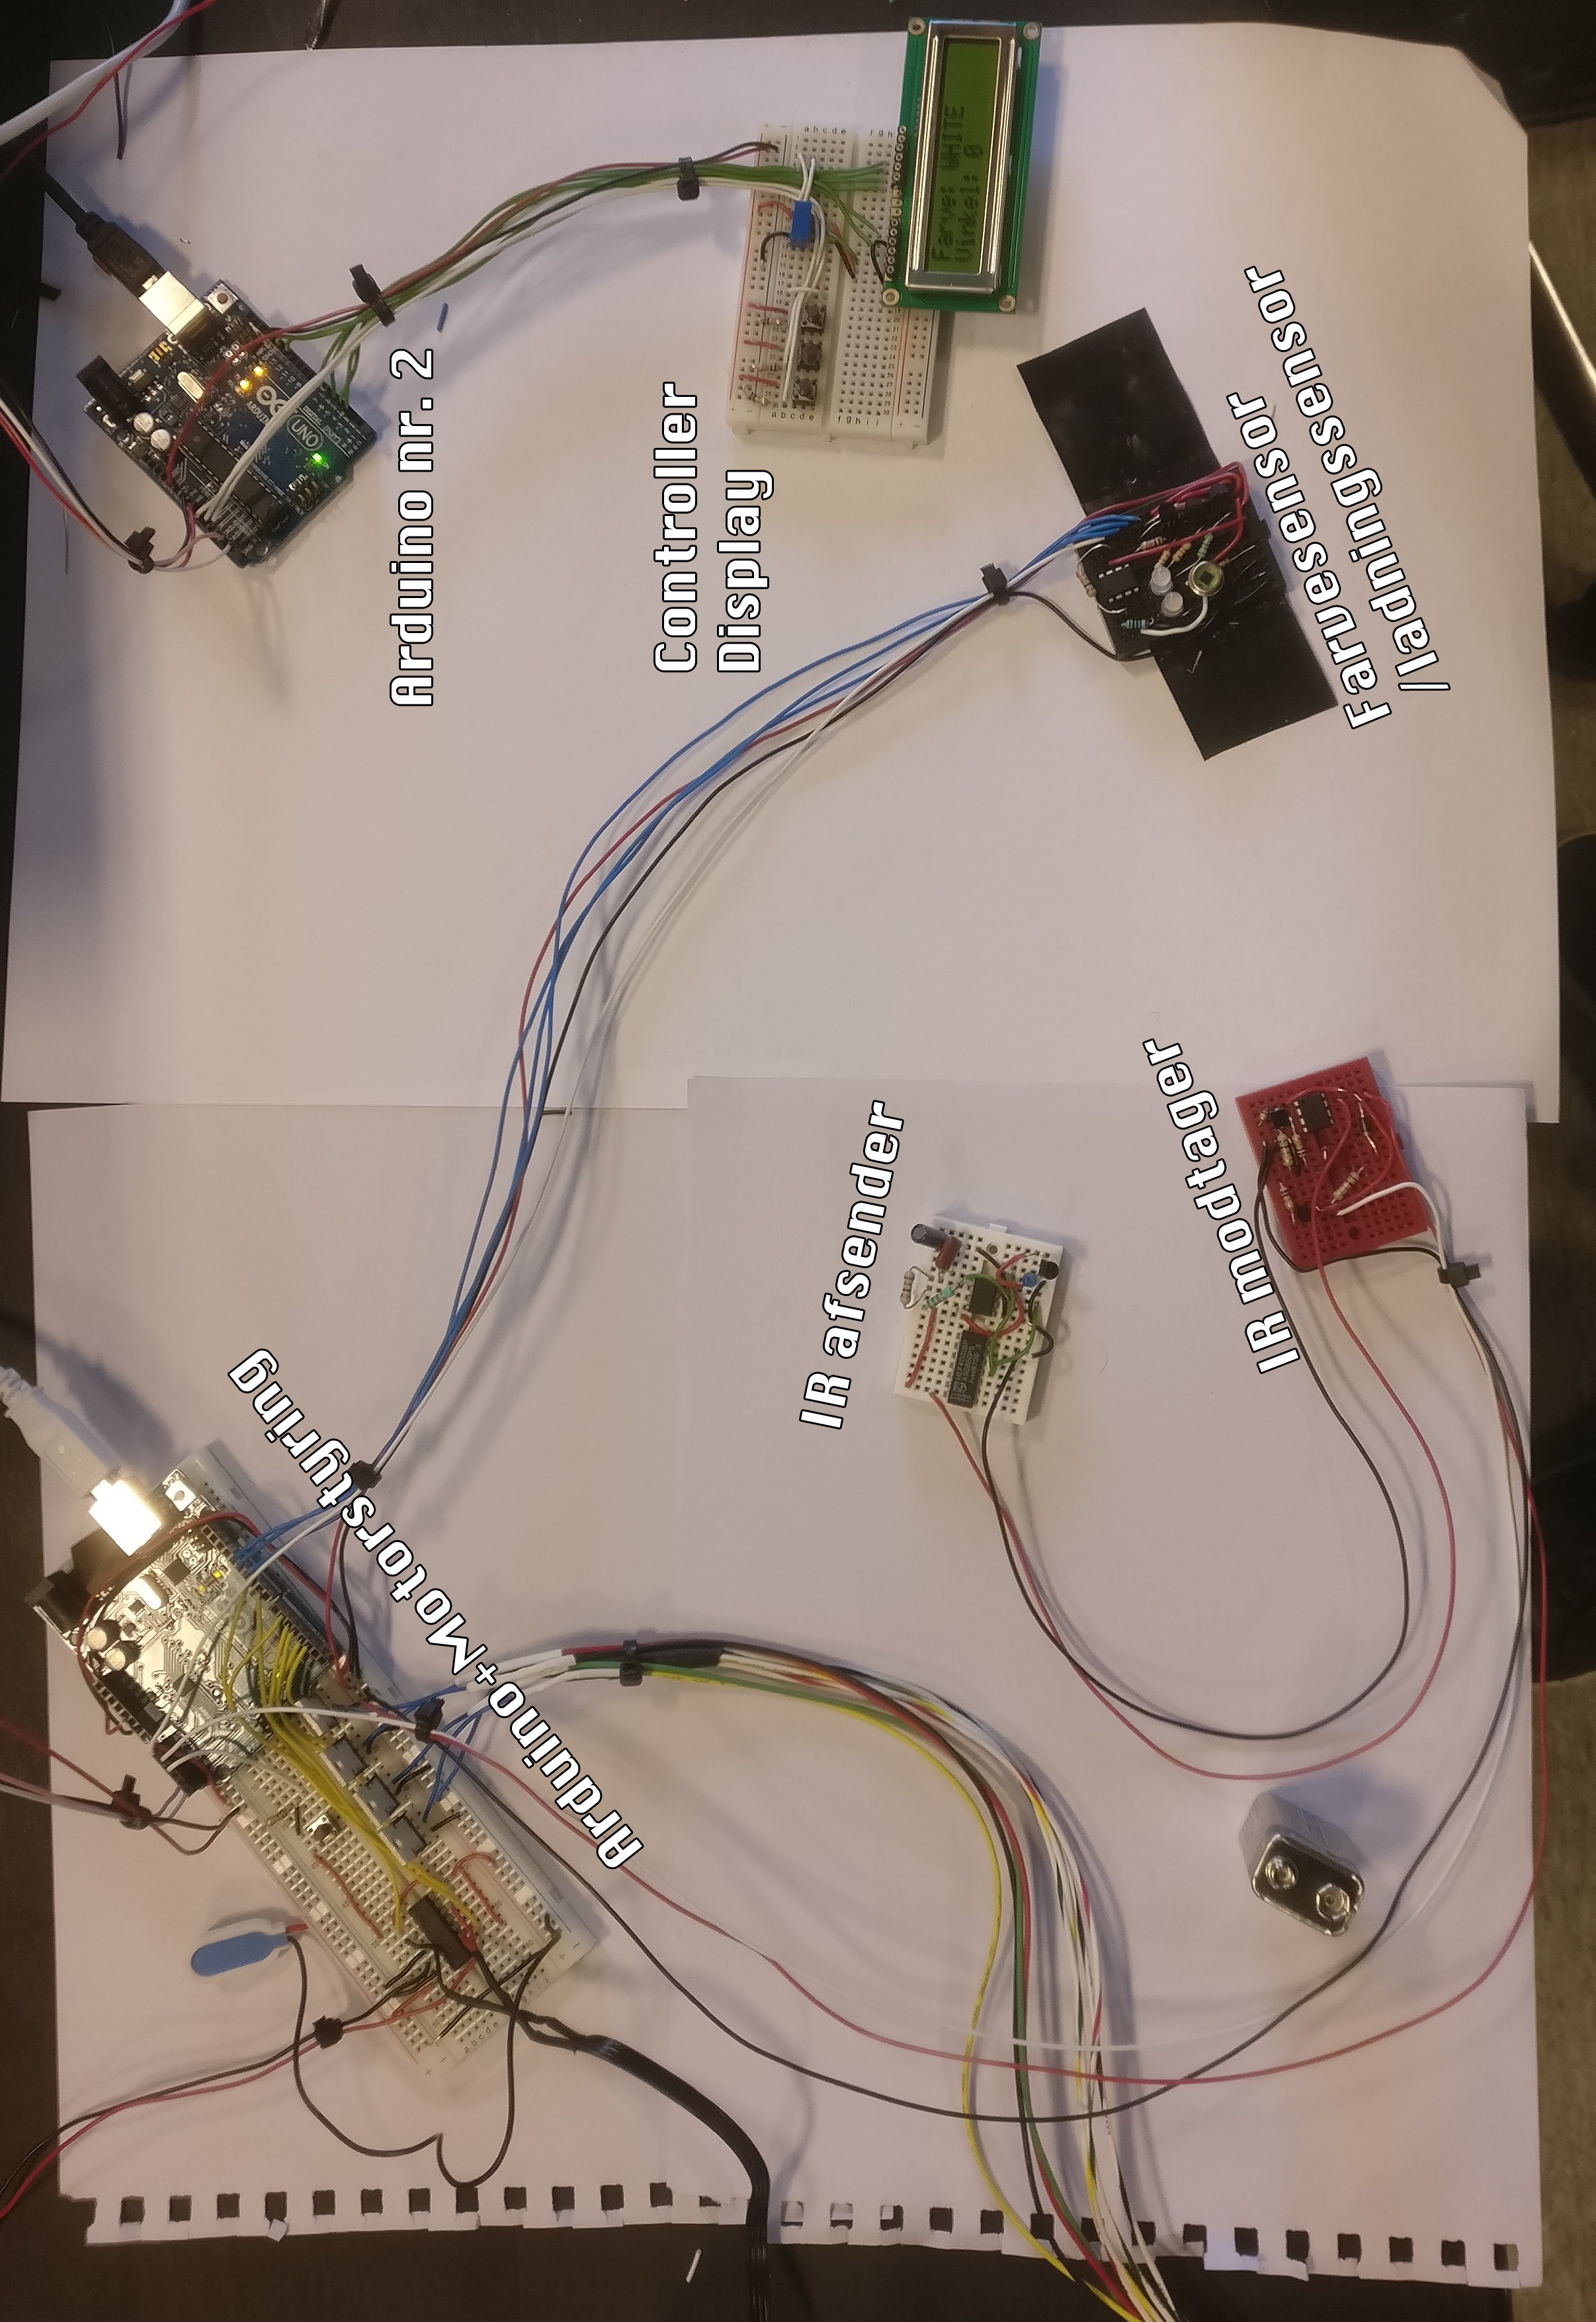
\includegraphics[width=15cm]{figures/2_5fremstilling/prototyper/Endeligproto.png}
\end{center}

\section{Endelig prototype - kanonkonstruktion} \label{bilag:endeligprotokanon}
\begin{center}
	\includegraphics[height=20cm]{figures/2_5fremstilling/prototyper/paenkanon.jpg}
\end{center}
\section{PCB artwork til hastighedssensor}\label{bilag:afsenderModtagerArtwork}
\begin{figure}[H]
	\centering
    \includegraphics[width=210mm]{figures/2_5fremstilling/afsenderModtagerArtwork.png}
\end{figure}


\section{PCB artwork til arduino shield} \label{bilag:shieldArtwork}
\begin{figure}[H]
	\centering
    \includegraphics[width=210mm]{figures/2_5fremstilling/shieldArtwork.png}
\end{figure}

\todo{Måske skulle vi overveje at lave et nyt billede med samlede kabler}
\begin{figure}[H]
\section{Fumlebrætmodel anden del}
	\centering
    \includegraphics[width=13cm]{figures/2_5fremstilling/prototyper/rumleKreds.png}
\end{figure}

% Must be second last (the longer the later)
\section{Program til Master Arduino}
\label{bilag:programMaster}
\begin{lstlisting}
#include <Wire.h>
#include <Stepper.h>

//Debug funktioner - Hvis debug er defineret vil der komme debug output til serial porten
#define DEBUG //Hvis debug er defineret. Den foerste funktion paa hver linje bliver erstattet med den anden funktion paa linjen, naar programmet bliver kompileret
#ifdef DEBUG
#define DEBUG_PRINTLN(x) Serial.println(x)
#define DEBUG_PRINTLNF(x,y) Serial.println(x,y)
#define DEBUG_PRINT(x) Serial.print(x)
#else //Hvis debug ikke er defineret. Her gaelder det samme, som betyder at funktionerne bliver fjernet
#define DEBUG_PRINTLN(x)
#define DEBUG_PRINTLNF(x,y)
#define DEBUG_PRINT(x)
#endif

//Wire - I2C protokol
int ADDRESS = 9; // Dens egen addresse. Ikke noedvendig, da dette er masteren af netvaerket, men blev sat alligevel
int SLAVEADD = 8; //Addressen til controlleren
char seperatorChar = 254; //ASCII tegnet som bruges til at adskille linjerne i dataen
char modeChar = 50; //ASCII tegnet som indikere at det en farve der skal paa displayet

//LCD variabler
char mode = 0; // Den sidste mode
String colorBuffer; //Den sidste sendte farve
String speedBuffer = "-1m/s"; //Den sidste sendte hastighed
String angleBuffer; //Den sidste sendte vinkel

//Retningsregulerende kreds
int stepperrev = 400; // Antal skridt per omgang
Stepper retning(stepperrev, 2, 3, 4, 5); //vores stepper motor objekt, med de tilsluttede ben og
int gearing = 40; //forholdet mellem hvor meget kannonen rygger sig og stepper motoren drejer
int stepsize = stepperrev * gearing / 180; // Skridtstoerrelsen for naar jystere, er lavet til at dreje 2 grad for hvert tryk
int currangle = 0; //Den nuvaerende vinkel i grader

//Controller
byte states; // det modtaget Port C input registre fra controlleren. Viser state af de forskellige ben
int upbit = 0; //Angiver hvilket bit i byten der tilhoere op knappen. analog A0
int downbit = 1; //Angiver hvilket bit i byten der tilhoere ned knappen. analog A1
int firebit = 2; //Angiver hvilket bit i byten der tilhoere skyd knappen. analog A2

//Hastighed
String Speed = "-1m/s"; //Den beregnede fart som string
int hastpin1 = A1; // Den ene hastighedsensor input ben
int hastpin2 = A2; // Den anden hastighedssensor input ben
float lengthtube = 1; //Laengden imellem de to hastighedssensor i meter

//Farver
boolean newball = true; //Angiver om der er kommet en ny bold i roeret, som betyder at farven skal tjekkes
int confirm; // Antallet af gange som sensoren har bestemt den samme farve
//Dette bliver brugt saa farven bliver bestemt flere gange i traek, og hvis det samme resultat kommer nok gange, antager vi at det den rigtige farve
int confirmAmount = 5; // Antallet af gange den skal faa den samme farve
int pinRGB[] = {12, 11, 13}; //benene til de forskellige LED'er
int pinColorSensor = A0; //Benet hvor farvesensoren er tilsluttet
int lightval[4]; //Et array til at gemme vaerdierne af farvesensoren naar den bliver belyst med forskellig farve. 0 er Roed, 1 er groen, 2 er blaa og 3 er hvid
int fireval = 0; //Angiver hvor haardt bolden skal skydes
String light[] = {"RED", "GREEN", "BLUE", "WHITE"}; //Angiver de forskellige farvers navne
String color; // Den sidste besluttede farve

//Affyringsmekanisme
int gearpinlock = 10; //Benet som vores gear laases paa
int gearpinunlock = 9; //Benet som vores gear laases op paa
int trekpin = 6; //Benet hvor vores traekke motor er paa. Skal kun kunne koere en vej

void setup() {
  //ben tilstanden saettes for vores input og output
  pinMode(gearpinlock, OUTPUT);
  pinMode(gearpinunlock, OUTPUT);
  pinMode(trekpin, OUTPUT);
  pinMode(pinRGB[0], OUTPUT);
  pinMode(pinRGB[1], OUTPUT);
  pinMode(pinRGB[2], OUTPUT);
  pinMode(pinColorSensor, INPUT);
  pinMode(hastpin1, INPUT);
  pinMode(hastpin2, INPUT);

  //Da vi benytter NPN transistor, skal benene saettes hoej for at slukke LED'erne
  digitalWrite(pinRGB[0], HIGH);
  digitalWrite(pinRGB[1], HIGH);
  digitalWrite(pinRGB[2], HIGH);

  //Kommunikationen med I2C starter, med angivet addresse
  Wire.begin(ADDRESS);

  //Serial kommunikation med computeren hvis DEBUG
#ifdef DEBUG
  Serial.begin(9600);
#endif

  //Hastigheden af vores retningsregulerende motor saettes (stepper motoren)
  retning.setSpeed(25);
}

void loop() {
  //Ser om den foerste hastighedssensor er blokeret, hvilket betyder at der er en bold i roeret.
  //Hvis der er det, saa bestem dens farve
  if ((analogRead(hastpin1)) <= 250)determinecolor();
  else {
    //Ellers nulstil vaerdier til naeste bold
    DEBUG_PRINTLN("WAITING FOR BALL");
    newball = true;
    confirm = 0;
  }
  getinput(); //Faa input fra controlleren
  lcddisplay(); //Hvis der er noget nyt der skal paa displayet, saa skriv det til controlleren
}


//Denne funktion modtager en byte fra controlleren, hvori at tilstanden af op, ned og skyd benet er i. Denne funktion finder ud af hvad der skal ske naar de forskellige er trykket
void getinput() {
  Wire.requestFrom(SLAVEADD, 1); //Anmoder om 1 byte data fra controlleren

  //Hvis noget data bliver sendt, saa set det i states
  if (Wire.available()) states = Wire.read();
  else return;

  //Udskriver hvad vi har modtaget binaert
  DEBUG_PRINT("Recieved: ");
  DEBUG_PRINTLNF(states, BIN);

  //Ser om op knappen er trykket, og ned knappen ikke er trykket
  if (bitRead(states, upbit) && !bitRead(states, downbit)) {
    //Hvis den er det, saa skal retningsmotoren koere 1 grad op
    DEBUG_PRINT("Updated angle from ");
    DEBUG_PRINT(angle()); //Funktion til at udskrive vinklen som en string
    DEBUG_PRINT(" to ");
    currangle += 2; //Aendre den nuvaerende vinkel med 2 grad
    DEBUG_PRINT(angle()); //Udskriver den nye vinkel
    DEBUG_PRINTLN();
    retning.step(stepsize); //Saetter retningsmotoren til at koere 2 grad op
  }
  //Ser om op knappen er trykket, og ned knappen ikke er trykket
  if (bitRead(states, downbit) && !bitRead(states, upbit)) {
    //Hvis den er det, saa skal retningsmotoren koere 1 grad ned
    DEBUG_PRINT("Updated angle from ");
    DEBUG_PRINT(angle());
    DEBUG_PRINT(" to ");
    currangle -= 2; //Aendre den nuvaerende vinkel med -2 grad
    DEBUG_PRINT(angle());
    DEBUG_PRINTLN();
    retning.step(-stepsize);//Saetter retningsmotoren til at koere 2 grad ned
  }
  if (bitRead(states, firebit))fire(); //Kalder affyringsfunktionen hvis skyd knappen er trykket
}

// Funktionen som skyder bolden afsted
void fire() {
  DEBUG_PRINTLN("Firing");
  if (!(analogRead(hastpin1) <= 250)) { //Hvis den ene hastighedssensor er hoej, saa er der ikke en bold i roeret, som betyder at affyringen skal stoppes
    DEBUG_PRINTLN("NOT LOADED");
    return;
  }
  if (newball) { //Hvis boldens farve stadig ikke er bekraeftet, saa stop affyringen
    DEBUG_PRINTLN("COLOR NOT VERIFIED");
    return;
  }
  //Skriver indstillingen (farven) til Serialporten
  DEBUG_PRINT("Setting: ");
  DEBUG_PRINTLN(color);

  long time = millis(); //den nuvaerende tid i millis
  digitalWrite(trekpin, HIGH); //Saetter traek bennet hoej, saa elastiken bliver strukket ud
  digitalWrite(gearpinlock, 130); //Saetter den i gear
  while (millis() - time <= fireval * 1000); // Treaker i det stykke tid der svare til indstillingen
  // Der laases nu op, ved at saette den i frigear
  DEBUG_PRINTLN("UNLOCKING");
  digitalWrite(gearpinlock, LOW);
  digitalWrite(gearpinunlock, 130); //traekker gearet ud i frigear
  digitalWrite(trekpin, LOW);

  time = millis(); //Vi opdatere tiden
  determinespeed(); //Funktionen der bestemmer boldens hastighed
  while (millis() - time <= 2000); //Saa laenge der ikke er gaaet 2 sekunder, saa vent, Dette er for at soerge for at gearet bliver holdt i frigear i lang nok tid
  digitalWrite(gearpinunlock, LOW); //Stopper med at holde gearet fast i frigear
}


String angle() { //Returnere vinklen som en string
  return String(currangle);
}

void determinecolor() {// Bestemmer farven af bolden i roeret
  if (!newball) return; // Hvis farven alleree er bestem og bekraeftet, saa lad vaere med at tjekke farven
  DEBUG_PRINTLN("DETERMINE COLOR");
  //Taender for alle farverne
  for (int i = 0; i < 3; i++) {
    digitalWrite(pinRGB[i], LOW);
  }
  delay(10);
  lightval[3] = analogRead(pinColorSensor); //gemmer farvesensorens vaerdi i lightval[3]
  //slukker alle LED'erne igen
  for (int i = 0; i < 3; i++) {
    digitalWrite(pinRGB[i], HIGH);
  }

  if (lightval[3] > 770) { //Hvis spaendingen er hoejere end 3.8 V er bolden hvid
    setColor(light[3], 1); //Saetter farven til hvid
    return;
  }

  for (int i = 0; i < 3; i++) {//Gaar igennem alle LEDerne og taender og slukker dem en efter en, og gemmer farvesensor vaerdien
    digitalWrite(pinRGB[i], LOW); //Taender for LEDen
    delay(10);
    lightval[i] = analogRead(pinColorSensor); //gemmer vaerdien i lightval
    DEBUG_PRINT(light[i]);
    DEBUG_PRINT(" Value: ");
    DEBUG_PRINTLN(lightval[i]);
    digitalWrite(pinRGB[i], HIGH); //slukker LEDen igen
  }

  if (lightval[0] * 1.2 > lightval[1] && lightval[0] * 1.2 > lightval[2]) { //Tjekker om farven er roed
    setColor(light[0], 2); //Saetter farven til roed og skydevardien til 2
    return;
  }
  if (lightval[1] > lightval[2] && lightval[1] > lightval[0]) { //Tjekker om farven er groen
    setColor(light[1], 3); //Saetter farven til roed og skydevardien til 3
    return;
  }
  if (lightval[2] > lightval[0] && lightval[2] > lightval[1]) { //Tjeker om farven er blaa
    setColor(light[2], 4); //Saetter farven til roed og skydevardien til 4
    return;
  }
}

void setColor(String newColor, int newFireval) { // Denne funktion saetter farven, og tjekker bekraeftelse
  if (color == newColor) {  //Hvis den forrige bold var samme farve, saa skal confirm blive 1 hoejere
    confirm += 1;
    if (confirm == confirmAmount)newball = false; //Hvis antallet af gange boldens farve er blevet bekraeftet, saa saet newball falsk
  } else { // Ellers genstart bekraeftelses processen og saet farven til newColor
    confirm = 0;
    color = newColor;
  }
  fireval = newFireval; //Tiden som elastikken skal blive traekket i bliver sat til newFireval
  DEBUG_PRINT("COLOR DETECTED : ");
  DEBUG_PRINTLN(color); //Skriver den fundede farve til Serialporten
}

void determinespeed() { // Bestemmer hastigheden af bolden
  DEBUG_PRINTLN("DETERMING SPEED");
  unsigned long time = millis(); //den nuvaerende tid saettes i time
  long calc; //en vaerdi til at se hvornaar den foerste hastighedssensor kan se bolden
  while (millis() - time <= 3000 && !(analogRead(hastpin1) <= 250)); //Venter til den foerste hastighedssensor bliver blokeret eller der er gaeet 3 sekunder
  calc = millis(); //saetter calc til den nuvaerende tid
  while (millis() - time <= 3000 && !digitalRead(hastpin2)); //Venter til den anden hastighedssensor bliver blokeret eller der er gaet 3 sekunder fra funktionen startede
  if (millis() - time >= 3000) { //tjekker om der er gaaet 3 sekunder, som betyder at der er TIMEOUT
    return;
  }
  Speed = String(lengthtube / (((float)(millis() - calc)) / 1000.0), 1); //Beregner hastigheden og laver det om til en String med 1 decimal precision
  Speed += "m/s";
  DEBUG_PRINTLN("Updated speed: " + Speed);
}

void lcddisplay() {//Opdatere displayet
  String data; //Stringen som skal sendes. Denne bliver bygget paa igennem funktionen
  boolean changed = false; //Angiver om noget har aendret sig paa displayet siden den sidst blev opdateret
  //Ser om farven har aendret sig
  if (colorBuffer != color) {
    mode = modeChar; //tilstanden bliver sat til farv
    data += mode; //saetter moden paa data stringen
    colorBuffer = color; //laver farve bufferen om til den nuvaerende farve
    data += colorBuffer; //saetter farvebufferen paa data stringen
    changed = true; //Angiver at noget har aendret sig
  }
  //Ser om hastigheden har aendret sig
  else if (speedBuffer != Speed) {
    mode = modeChar + 1; //tilstanden bliver sat til hastighed (noget andet end modeChar)
    data += mode; //Saetter moden paa data stringen
    speedBuffer = Speed; //Laver hastighedsbufferen om til den nuvaerende hastighed
    data += speedBuffer; //Saetter hastighedsbufferen paa data stringen
    changed = true; //angiver at noget har aendret sig
  } else { //Ellers fyldes data stringen op med de sidst gemte vaerdier. Detter er vist anden linje skal opdateres
    data += (char)mode;
    if (mode == modeChar)data += colorBuffer;
    else data += speedBuffer;
  }
  data += seperatorChar; //Saetter en seperator paa enden af data stringen
  if (angleBuffer != angle() || changed) {// Hvis vinklen ikke er den samme eller hvis foerste linje har andret sig
    angleBuffer = angle(); //Saetter vinkelbufferen til den nuvaerende vinkel
    data += angleBuffer; //Saetter vinkelbufferen paa data stringen
    changed = true; //Angiver at noget har aendret sig
  }
  data += seperatorChar;//Saetter endnu et seperationstegn
  if (changed) { //Hvis noget har aendret sig
    DEBUG_PRINT("TRANSMITTING: ");
    DEBUG_PRINTLN(data);

    //Laver data stringen om til et array af char
    char dataBuffer[data.length()];
    data.toCharArray(dataBuffer, data.length());

    //Begynder kommunikation til controlleren, og overfoere dataen som et char array
    Wire.beginTransmission(SLAVEADD);
    Wire.write(dataBuffer);
    Wire.endTransmission();
  }
  delay(100); //Venter i 0.1 sekund for at forhindre overbelastning af I2C bufferen
}
\end{lstlisting}

\section{Program til Controller Arduino}
\label{bilag:programController}
\begin{lstlisting}
#include <LiquidCrystal.h>
#include <Wire.h>


//Debug funktioner - Hvis debug er defineret vil der komme debug output til serial porten
#define DEBUG
#ifdef DEBUG //Hvis debug er defineret. Den foerste funktion paa hver linje bliver erstattet med den anden funktion paa linjen, naar programmet bliver kompileret
#define DEBUG_PRINTLN(x) Serial.println(x)
#define DEBUG_PRINTLNF(x,y) Serial.println(x,y)
#define DEBUG_PRINT(x) Serial.print(x)
#else //Hvis debug ikke er defineret. Her gaelder det samme, som betyder at funktionerne bliver fjernet
#define DEBUG_PRINTLN(x)
#define DEBUG_PRINTLNF(x,y)
#define DEBUG_PRINT(x)
#endif

//Wire - I2C protokol
int ADDRESS = 8; // Dens egen addresse. Denne skal bruges naar master vil kontakte controlleren
char seperatorChar = 254; // ASCII tegnet som bruges til at adskille linjerne i dataen
char modeChar = 50; //ASCII tegnet som indikere at det en farve der skal paa displayet

//knapper til controlleren. Benene bliver kun brugt til at angive at det er input, ellers benyttes port manipulation (PINC) til at sende benenes tilstande som en byte.
int uppin = A0;
int downpin = A1;
int skydpin = A2;

//LCD variabler
LiquidCrystal lcd(12, 11, 5, 4, 3, 2); //vores LCD objekt, med benene som den er koblet paa
String line1_const1 = "Farve: "; //Den ene konstant paa linje 1. Skal have et mellemrum efter, da .length bliver brugt
String line1_const2 = "Fart: "; //Den anden konstant paa linje 1. Der skiftes mellem disse med mode i modtager funktionen
String line2_const = "Vinkel: "; //Den ene konstant paa linje 2.


void setup() {
  //ben tilstand for knapperne saettes som input
  pinMode(uppin, INPUT);
  pinMode(downpin, INPUT);
  pinMode(skydpin, INPUT);

  //Starter I2C kommunikation
  Wire.begin(ADDRESS); //Angiver addresse og begynder
  Wire.onRequest(requestEvent); //Angiver funktion der skal kaldes naar controlleren bliver bedt om at sende
  Wire.onReceive(receiveEvent); //Angiver funktion der skal kaldes naar controlleren skal modtage

  //Starter LCD
  lcd.begin(16, 2); //Begynder LCD'en med 2 linjer og 16 tegn per linje
  lcd.print(line1_const1); //Skriver 1. linje konstant paa LCD
  lcd.setCursor(0, 1); //Skifter position til 2. linje
  lcd.print(line2_const); //Skriver 2. linje konstant paa LCD

  //Starter serialkommunikation hvis DEBUG er defineret
#ifdef DEBUG
  Serial.begin(9600);
#endif
}
// Loop funktionen, controlleren skal ikke goere noget hvis den ikke bliver bedt om det
void loop() {
}

//Naar controlleren skal sende data
void requestEvent() {
  byte data = PINC; //Port C input registret
  //Skriver den sendte data binaert i serialkommunikationen hvis DEBUG er defineret
  DEBUG_PRINT("TRANSMITTING DATA: ");
  DEBUG_PRINTLNF(data, BIN);
  DEBUG_PRINTLN();

  Wire.write(data); //Sender dataen over I2C
}

//Naar controlleren modtager data
void receiveEvent(int datalength) {
  DEBUG_PRINTLN("RECIEVING DATA: ");

  boolean mode = (Wire.read() == modeChar ); //Den foerste byte indikere tilstand, hvor at den enden kan vaere 0 eller hoejere end 0

  //Stringene for den 1. og 2. linje
  String firstLineBuffer = getLine(); //Faar den 1. linje fra I2C bufferen
  String secondLineBuffer = getLine(); //Faar den 2. linje fra I2C bufferen

  setDisplay(mode, firstLineBuffer, secondLineBuffer); // Det modtaget data bliver sendt til funktionen setDisplay, som skriver dataen til displayet
}

//Denne funktion laeser fra I2C bufferen indtil at den er tom eller at ny linje tegnet dukker op. Dette bliver sat i en String som bliver returneret
String getLine() {
  String output;
  while (Wire.available()) {//Saa laenge der er noget i I2C bufferen
    char c = Wire.read(); //laes det naeste tegn
    if (c == seperatorChar) break; //Hvis tegnet er seperationstegnet, stop med at laese fra bufferen
    DEBUG_PRINT(c); //Skriv til Serial hvis DEBUG
    output += c; //Ellers skal tegnet tilfoejes til output
  }
  DEBUG_PRINTLN();
  return output; //returner outputtet
}

//opdatere displayet
void setDisplay(boolean mode, String line1, String line2) {

  //Debug udskrivning. Skriver hvad displayet bliver opdateret til
  DEBUG_PRINT("Updating display:  ");
  DEBUG_PRINT("Line 1: ");
  DEBUG_PRINT(line1);
  DEBUG_PRINT("    ");
  DEBUG_PRINT("Line 2: ");
  DEBUG_PRINTLN(line2);
  lcd.clear(); //Fjerner alt fra displayet
  lcd.setCursor(0, 0); //Saetter position til starten af displayet paa 1. linje
  int leng; //laengde paa 1. linje. Dette bruges til at goere resten af felterne tomme paa linjen tomme

  // Skriver konstanten paa 1. linje, alt efter hvilken mode det er (hastighed/farve)
  if (mode) {
    lcd.print(line1_const1);
    leng += line1_const1.length();
  }
  else {
    lcd.print(line1_const2);
    leng += line1_const2.length();
  }

  lcd.print(line1); // Skriver dataen til linje 1 paa linje 1.
  lcd.setCursor(0, 1); // Saetter positionen til 2. linje efter konstanten
  lcd.print(line2_const);
  lcd.print(line2); //Skriver dataen til linje 2 paa linje 2.
}
\end{lstlisting}



% MUST BE LAST
\includepdf[pages = 1, pagecommand = \section{Logbog} \label{bilag:logbog}]{figures/logbog.pdf} 
\includepdf[pages = 2-, pagecommand={}]{figures/logbog.pdf} 


\end{document}



